\section{Zickzack}
Das Verfahren konvergiert oftmals sehr langsam, da es sich dem Optimum
entweder mit einem starken Zick-Zack-Kurs n"ahert oder der Betrag des
Gradienten in der N"ahe des Optimums sehr klein ist, wodurch die L"ange
der Iterationsschritte dann ebenfalls sehr klein ist.

\begin{figure}[htb]
\centering
\begin{subfigure}[b]{0.49\textwidth}
\centering
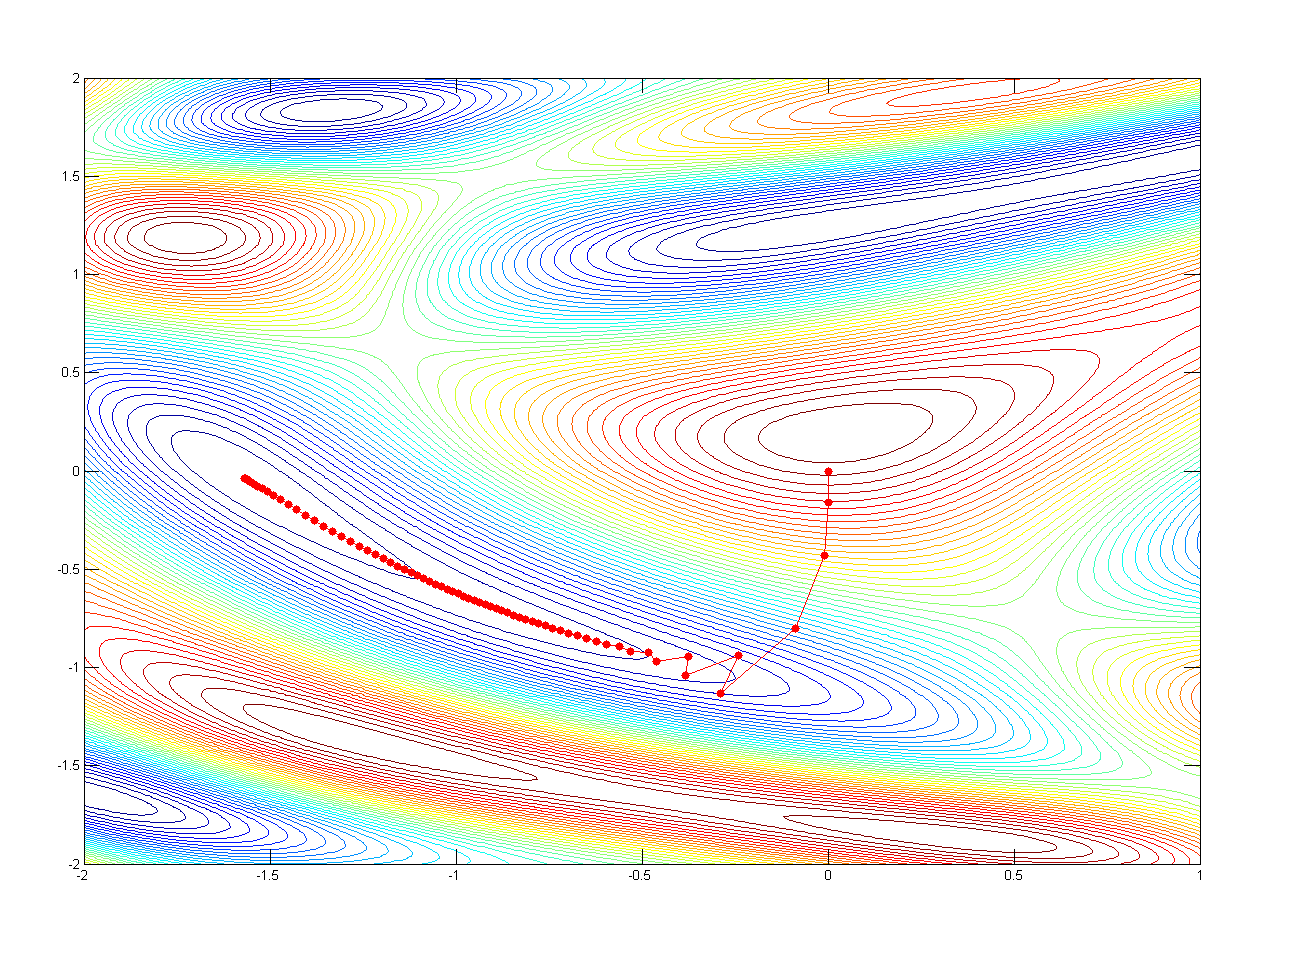
\includegraphics[width=\textwidth]{descent/zz_3.png}
\caption{leichtes Zickzack und kleine Iterationsschritte}
\end{subfigure} \begin{subfigure}[b]{0.49\textwidth}
\centering
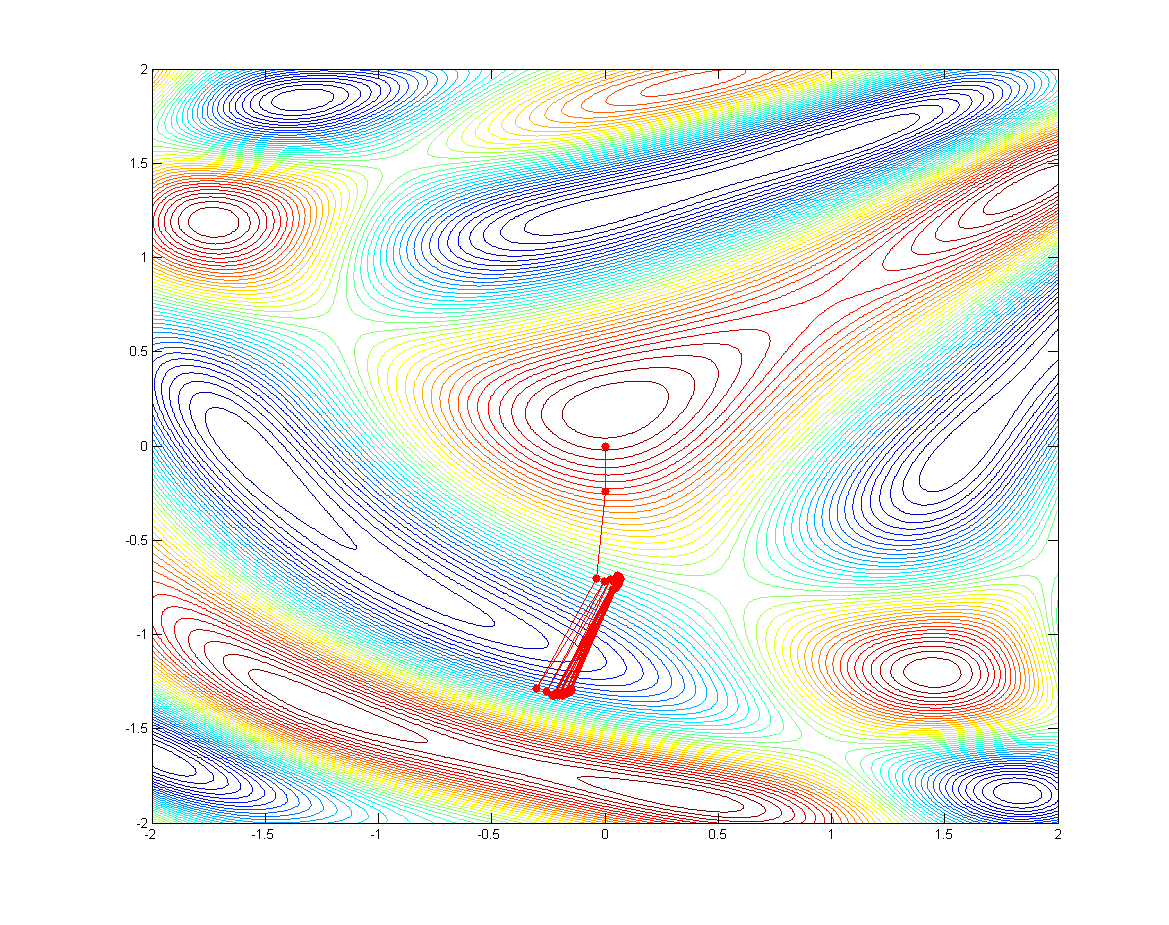
\includegraphics[width=\textwidth]{descent/zz_2.png}
\caption{Starkes Zickzack}\label{zickzackb}
\end{subfigure}
\caption{Verschiedene Zickzack}\label{zickzack}
\end{figure}

Bei gewissen Raumstrukturen kann das ZickZack vorkommen. Bei einem
leichten ZickZack ist die Zielfindung gegeben, aber mit h"oherem
Arbeitsaufwand verbunden.
Beim Extremfall ist eine genaue Ann"aherung an das Ziel nicht m"oglich,
da der Algorithmus in einer Endlosschleife feststeckt.
In \figref{s_vs_i} ist der Extremfall im Bereich der Schrittweite 0.15
klar sichtbar.

\begin{figure}
\centering
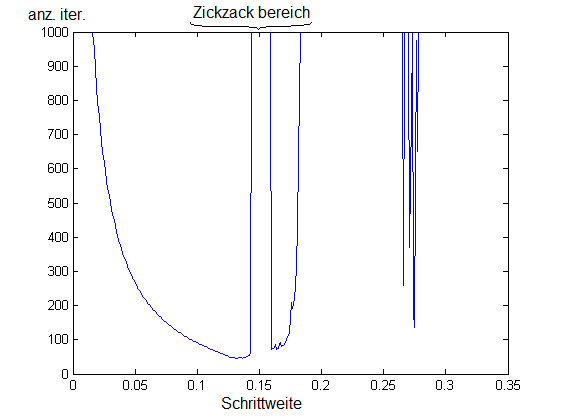
\includegraphics[height=0.5\textwidth]{descent/zzstep.png}
\caption{Schrittweite zu Iterationsschritten}\label{s_vs_i}
\end{figure}


